\documentclass[10pt,letterpaper]{article}
\usepackage[margin=1in]{geometry}
\usepackage[T1]{fontenc}
\usepackage{lmodern,microtype,amsmath,amssymb,amsthm,booktabs,array,graphicx,xurl}
\usepackage[hidelinks]{hyperref}
\microtypesetup{protrusion=false}
\newtheorem{theorem}{Theorem}
\newtheorem{proposition}[theorem]{Proposition}
\newtheorem{lemma}[theorem]{Lemma}
\newcommand{\F}{\mathcal F}\newcommand{\C}{\mathcal C}\newcommand{\D}{D^\star}
\newcommand{\ind}{\mathbf 1}\newcommand{\dist}{\operatorname{dist}}
\setlength{\emergencystretch}{2em}
\title{Technical Supplement: Exact Joint Deformation and\\ Conditional Count Bounds in Ordered Cell Corridors}
\author{Arnav Peram}\date{}
\begin{document}\maketitle
This supplement develops the auxiliary exact representation, standard consequences and software diagnostics supporting the main paper. The complete ownerwise representation proof appears in the main paper, so it does not depend on an unpublished predecessor. Native results quantify local conditional families; generated examples assess implementation and mechanisms.
\section{Exact critical-mesh reduction and the direct representation}
The canonical-realization lemma also supplies an exact finite-height route. The implementation is an exact reference construction using a shared integer-flow backend. Standard ordered-surface cuts supply the finite backend once sufficient candidates and costs have been derived.

\subsection{An ownership-independent common mesh}
Collect on each boundary every possible propagated lower/upper obligation term, fixed band/endpoint term, and source piece. Form a common mesh from their piece endpoints and every same-boundary isolated crossing. These are physical-input events, chosen before owners or molecular costs. Identical pieces do not create infinitely many crossings.

\begin{proposition}[Critical-mesh ownerwise equality]
For the absolute-displacement objective, restricting nodal heights to candidate-function values on this mesh, with the original constraints and trapezoidal nodal costs, preserves both feasibility and $D^\star(c)$ for every owner vector $c$.
\end{proposition}
\begin{proof}
Between mesh events every candidate piece is affine, candidate ordering is fixed, and all crossings with the source are included. Every canonical lower/upper envelope and clamp therefore selects affine pieces with constant-sign displacement. Its trapezoidal area is exact, and every nodal value is an available candidate. Thus a canonical minimizer for each feasible $c$ is retained at cost $D^\star(c)$.

Conversely, any feasible nodal candidate family interpolates to a continuous feasible family: the common mesh includes all source and obligation endpoints, and the slope, band, separation and interval-ownership constraints are linear between nodes. Absolute displacement on each affine interval is convex; its trapezoid upper-bounds its integral. That integral is at least $D^\star(c)$. The retained canonical realization gives the reverse inequality. Both directions prove the statement. Exactness of trapezoids is asserted for the canonical absolute displacement, not for every interpolant or arbitrary nonlinear loss powers.
\end{proof}

For candidates $v_0<\cdots<v_\ell$ at a surface/node pair, encode $H_k=\mathbf1[h\ge v_k]$, $k\ge1$, with $H_{k+1}\Rightarrow H_k$. The minimum candidate is unconditional. For $h_b\ge h_a+d$, every origin threshold implies the first destination threshold at least $v_k+d$; a missing destination forces the origin false. This includes the unconditional minimum constraint. Both directions enforce slopes and finite gap bounds. For an owner bit $b$, $b\Rightarrow h\ge L$ is a threshold implication, and $(b=0)\Rightarrow h\le U$ is its contrapositive $H_{\text{first value}>U}\Rightarrow b$. Apply obligations at every mesh node in their intervals. Trapezoidal absolute displacement and molecular terms are unary ordered-label costs, encoded by successive differences and constant shifts. Integer scaling gives an exact cut.

\subsection{Pruning, scope and graph size}
The reference gets the same ownership/pin closure as the direct compiler. Fixed-inactive cones are omitted. Fixed-active and geometric constraints give lower/upper envelopes which contain every feasible height. Crossings and candidates outside that interval are irrelevant to every canonical minimizer and are omitted. This is not a reward-dependent mesh. If all owners are forced, the reference reconstructs their canonical realization and skips height expansion; this also handles positive mandatory deformation.

Let $P$ count candidate affine pieces, $Q=O(P^2+P)$ the common event count, and $H=\sum_{b,j}(|V_{bj}|-1)$ the retained height bits. The reference graph has $Gm+H+2$ vertices and $O(H+NmQ+Gm)$ arcs, plus the retained redundant ownership-closure arcs. Candidate sorting and rational capacity scaling are polynomial. The direct graph instead retains molecular bits and merged integrated activation helpers. Neither formula implies a universal dominance or minimal graph-size theorem. This compares the explicit constructions, rather than every possible compressed surface graph.

At zero area penalty, a height-graph optimum need not be the least-area realization of its owners; area is unpenalized. It still attains the requested objective. Pinned ownerwise-area verification uses area coefficient one. The source-clipping shortcut and singleton upper bound require zero-deformation admissibility of every source ownership obligation, whereas the general representation permits source-inconsistent universal regions.


\section{Prefix-family aggregation: a tighter graph-size bound}
For one output boundary and polarity, let $M$ count propagated untruncated terms
\[
 g_i(t)=\alpha_i-s_i\dist(t,I_i).
\]
The positive excursion is $[g_i(t)-r(t)]_+$, with a common piecewise-affine reference $r$; using $r=-f^0$ covers the other polarity. The same argument applies after pin substitution replaces $r$ by a mandatory envelope.

\begin{proposition}[Quadratic prefix-family bound]
After merging identical activation sets, $O(M^2+M)$ helper vertices and helper arcs suffice for this boundary/polarity, independently of the number of reference knots. Across all boundaries, the main-text vertex and arc bounds follow, with auxiliary contribution $O(N^2m^5)$ when $M_b=O(Nm^2)$.
\end{proposition}
\begin{proof}
Each $g_i$ has at most three affine pieces. For a pair, their combined breakpoints split the domain into at most five intervals; on each their difference is affine. Hence their ordering changes only constantly many times, including transitions into and out of coincidence intervals. Choose a fixed index tie rule on every open interval. Consecutive orderings differ by adjacent swaps, with the total number of swaps bounded by the total pair-order changes, $O(M^2)$. A block of simultaneous crossings can be expanded into such swaps for counting; hypothetical intermediate prefixes only enlarge the family and preserve the upper bound.

One ordering has at most $M$ nonempty cone-index prefixes. An adjacent swap changes just the prefix ending between the swapped positions. Thus the union of all prefixes has size $O(M^2+M)$. The common reference changes which terms are positive but not their relative order: the positive terms are an initial segment of the same ordering. Every nonzero layer therefore uses one of the counted prefixes. Mapping cone indices to their activation labels cannot increase the number of distinct sets, even when several cones carry the same bit.

For each new activation set $S$, choose an occurrence of its prefix and the last newly appearing label $v$ there. The preceding distinct-label prefix is $P=S\setminus\{v\}$. Retain $P$ even if its aggregate weight is zero, and connect its helper and $v$ to the helper for $S$ (reverse the implications for complement polarity). Cardinalities strictly decrease down predecessor links, so the construction is acyclic and uses constant arcs per set. Every required predecessor is another prefix in the same counted family; no additional asymptotic factor appears. Sum exact weights from every slab and every repeated occurrence.

Summing over both polarities and all destinations gives $O(\sum_b(M_b^2+M_b))$ helpers. Owner bits add $O(Gm)$ vertices; nesting, unary pins and ownership implications add $O(Gm+N^2m^2)$ arcs. This proves the stated graph-size bound.
\end{proof}

This is an existence/aggregation bound, not a kinetic construction-time theorem. Source knots and zeros may generate many integration slabs; the present implementation scans layers before merging. Source geometry also changes integrated rational weights and their bit lengths. No lower bound for all compressed height encodings is asserted. New rational checks cover 168 polarity-arrangements, 1,260 activation assignments and 484 predecessor-helper identities, including simultaneous events, coincident functions, repeated labels and 41-knot oscillatory references. Test truth integrates selected maxima separately from the production layer routine.

\section{Source-clipped completion and targeted spectra}
The main paper requires that the source satisfies every source-owner obligation, including structural pins and universal site regions. Here is the full closure argument. In a finite implication system, let $T$ be the forward closure of all forced-one vertices and $F$ the reverse closure of all forced-zero vertices. An intersection proves infeasibility. Otherwise the assignment with ones exactly $T$ is the least feasible pinned vector, and the assignment with zeros exactly $F$ is the greatest. Clipping the feasible source vector between these extremes preserves every implication, since the set of implication-satisfying vectors is closed under coordinatewise minimum and maximum.

Every selected obligation retained from the source produces zero positive source-relative excursion. Every changed bit of the clipped vector is forced, and therefore every feasible pinned completion activates the same new excursion. A further optional change can only add to the relevant positive or negative maxima. Thus the clipped boundary is pointwise nearest among pinned completions and minimizes integrated deformation. The same reasoning shows that all changed molecular groups in this completion are necessarily changed in every other completion; consequently it minimizes the total nonnegative weight of changed groups as well.

For a query depending on $r$ groups, enumerate the $(m+1)^r$ target assignments, reject inconsistent closures, and record each completed score and its least area. Every feasible full assignment projects to one enumerated target vector; completion weakly reduces its area while preserving the score. Conversely every retained completion is attained. This proves exactness of the target spectrum. A limit reached before exhaustive coverage must yield an unresolved spectrum rather than an exact one.

\section{Two-resource bounds and joint predicates}
Let $H(c)=\sum_i w_i\ind[c_i\ne c_i^0]$ be a reassignment count or nonnegative integer weight. For budgets $D^\star(c)\leq\delta$, $H(c)\leq K$ and multipliers $\mu,\nu\geq0$, define
\[
m_+(\mu,\nu)=\min_c\{\mu D^\star(c)+\nu H(c)-S(c)\}.
\]
Then $S(c)\leq\lfloor\mu\delta+\nu K-m_+(\mu,\nu)\rfloor$ for every feasible $c$, by rearranging the defining inequality. Apply the same inequality to $-S$ for a lower bound. The count-weighted term is unary and therefore uses the same ownerwise representation.

Under source admissibility, the source-clipped completion above jointly minimizes area and reassigned weight for fixed target pins. Recording both resources for each target vector gives exact two-resource query spectra. This conclusion uses the special completion property; arbitrary pairs of resources need a Pareto frontier. Twenty generated models give 80 checked exact spectra and 480 sound bounds in the archived tests.

For multiple target counts, retain the joint tuple and least area, rather than taking the Cartesian product of marginal intervals. A predicate is always true, always false or variable according to all budget-feasible tuples. The enlarged three-cell native corridor c8f8188430d092 at area $4\,\mu$m$^2$ allows MDM2 in right cell 153965 and TFPI in left cell 153959 individually, each over $[0,1]$, but excludes their simultaneous presence under the stated thickness bound. This is a geometric conjunction, not evidence for or against signaling.

\section{Penalized optima and parameter paths}
For one fixed penalized graph, its optimal residual network represents every minimum cut: a source-side set is minimum exactly when it contains the source, excludes the sink, and is closed under positive residual arcs. Contracting residual strongly connected components gives the classical Picard--Queyranne description \cite{picard}. A candidate owner occurs in an optimum exactly when reachability from its required-one vertices and the source avoids the required-zero vertices and sink. Marginal owner domains need not form a feasible Cartesian product, and they describe penalized optima rather than all hard-budget assignments.

A monotone parametric cut requires the prescribed source/sink capacity directions and parameter-independent internal arcs \cite{gallo}. Extreme-cell nonnegative rewards can meet this condition after scaling $D-tN$. Middle-cell indicators equal the difference of two thresholds and can change opposite unary signs; nestedness therefore needs checking. The artifact includes an explicit nonnested example. Repeated exact cuts remain valid without a nested-path claim.
\section{Beyond one corridor: composition and a conservative raster model}
\subsection{Independent editable patches}
Local spectra can be combined when editable patches have disjoint interiors and observations, fixed traces at their boundaries, and connected local cell pieces attached to compatible connected fixed cores. These conditions imply a valid global partition and additive deformation. They must be established for the application; the overlapping native corridors in this study are not automatically gluable.

\begin{proposition}[Exact composition]
For independently gluable patches with local spectra \(d_j\), the global minimum cost at total count \(v\) is
\[
 d_{\rm global}(v)=\min_{v_1+\cdots+v_p=v}\sum_{j=1}^p d_j(v_j).
\]
\end{proposition}
\begin{proof}
Restrict a global assignment to obtain the lower bound. Conversely, local attaining assignments for a minimizing tuple glue under the stated conditions and achieve its sum.
\end{proof}
Ordinary sparse min-plus convolution computes this table. A direct dynamic program is polynomial in an explicitly bounded count range, but not automatically in the bit length of large multiplicities. Binary-encoded multiplicities can encode a knapsack problem; that encoding provides no hardness conclusion for explicitly listed unit transcripts or general planar tessellations. We make no such general hardness claim.

\subsection{A different uncertainty metric permits arbitrary label topology}
Let a 2D or 3D reference label image be \(c_0(x)\), and assume one common label-transport map \(\phi\) with \(\|\phi-\mathrm{id}\|_\infty\leq r\). A point can only inherit a label occurring within radius \(r\) of its location; localization radius \(e\) enlarges this to \(r+e\). Taking all intersecting voxel labels yields a conservative candidate set. Dropping common-map consistency gives a tractable outer family with arbitrary cell adjacency.

For a cell/gene, let \(n\) be its original count, \(a\) the number of its molecules that can leave, and \(b\) the possible incoming molecules. At a global unit-RNA change cap \(K\), the independent-label extrema are
\begin{equation}
 [n-\min(K,a),\ n+\min(K,b)].\label{eq:outer}
\end{equation}
Each endpoint follows by selecting the allowed departures or arrivals. Thus (\ref{eq:outer}) is exact for this relaxation and sound for a contained coherent geometry. Candidate extraction and sparse accumulation are implemented for 2D/3D integer label arrays in supplied physical coordinates. Crop-edge windows retain every known label plus an unknown-exterior label.

This extends \emph{coverage of a conservative model}, not exact connected segmentation. The displacement radius \(r\) and area budget \(\delta\) are different quantities. We do not transfer calibration or runtime claims between them.

\section{Calibration and statistical interpretation}
Fit the geometric family on training units only. Let a paired calibration region provide an aligned reference owner vector \(Y\), and score it by \(A(X,Y)=\D_X(Y)\), or infinity if it has no realization. The score concerns assignment representability, not necessarily the actual membrane's area; mismatches with fixed exterior assumptions also count as model failures. For \(n\) calibration units, choose the padded order statistic of rank
\(\lceil(n+1)(1-\alpha)\rceil\).

\begin{proposition}[Standard split-conformal consequence]
With unrestricted assignment fallback for an infinite threshold, and conditional on an independently trained family, exchangeability of calibration and test regions gives owner-vector coverage at least \(1-\alpha\) at that threshold. Every sound cell--gene interval propagated from the same set simultaneously covers its test count with at least that probability.
\end{proposition}
\begin{proof}
The standard split-conformal rank argument bounds the probability that the new score exceeds the padded quantile \cite{conformal}. On the complementary event, one included owner vector determines all true counts. Every sound interval contains those counts, so no additional union bound over entries is required.
\end{proof}
Infinite model-miss scores are retained. An infinite threshold requires an unrestricted assignment fallback or abstention from a finite geometric certificate. The guarantee is marginal over calibration and test units, not conditional accuracy for each donor. Calibration against another segmenter targets that reference, not unobserved anatomy. The current biological-data budgets are sensitivity settings; their probabilistic coverage has not been measured.

Fixed-weight contrasts can be optimized directly, but stability of their sign is different from statistical differential expression. A simultaneous count-set coverage statement alone does not produce valid differential-expression p-values or false-discovery-rate control. Those require a separately specified inferential procedure.

A discrete profile distribution proportional to \(\exp(-\lambda\D(c)+\text{utility})\) is also distinct from integrating a prior over continuous boundaries. Unary perturb-and-MAP is generally approximate \cite{papandreou}; our diagnostic retains its measurable discrepancy from the enumerated profile law. Neither randomized cuts nor an area penalty supplies calibrated assignment probabilities by declaration.

\section{Generated calibration diagnostics}
Thirty generated paired-boundary training units determine the slope and band; 99 independently generated calibration units determine the 90\% threshold. All seeds and rules precede these outcomes. On 200 independently generated test units, 184 complete owner vectors and 185 complete count matrices are covered. Simultaneous count coverage is 92.5\%, with a Wilson 95\% interval of 88.0--95.4\%; mean marginal interval width is 0.71. The source point-count matrix is correct in 97 units. A guard experiment retaining 20 incompatible calibration units correctly returns an unbounded threshold.

These are known synthetic assignments on piecewise-linear boundaries, not a realistic image simulator, independent tissue or a run of deployed segmenters. Pooled transcript AUROC is 0.8655 for exact reassignment fragility and 0.8612 for distance to the flat source. The small difference and within-region dependence do not establish superiority. Calibration coverage does not establish biological fidelity.

\section{Raster and engineering diagnostics}
The raster relaxation processes all 7,370 measured crop transcripts at radii 0,0.25,0.5 and 1$\mu$m, with explicit conservative treatment of crop-edge windows. It accepts 2D/3D arrays; 908 generated transport-membership checks pass. The streaming count routine is verified against exhaustive independent assignments on 120 small instances, and its C++ implementation matches 12,668 cross-language count entries.

For precomputed candidate lists, three fresh processes give a median 0.341-second time to read, accumulate and write candidate records at one million synthetic RNA records and 6.5 MiB peak resident memory. This excludes label-neighborhood construction, geometry, images and segmentation. It is not a whole-slide timing. The optional C++ flow backend uses arbitrary-precision integers and fresh standard Dinic flows; 100 exhaustive graph optima, including 10 huge-capacity cases, and 252 archived native objectives agree. No dynamic-flow or production-maxflow speed claim is made.


\section{Native count census and interpretive checks}
The native table uses 899 local cell--gene questions per geometry, eight area budgets and two geometries, giving 14,384 intervals. The 1,798 question definitions include 1,584 with only one local transcript of that gene. This small target multiplicity explains the tractability of exact projection and limits the evidence for a joint-count advantage. Source counts incorporate retained crop observations outside each selected corridor as fixed offsets. Those offsets do not authorize deformation elsewhere on the cell.

The separately executed checker reconstructs all target spectra with the older scanning compiler and late owner pins, rather than the new target-spectrum implementation. It agrees on all 14,384 endpoints and replays 1,176 stored root flow proofs. This is independent implementation-path evidence within one project. Complete marginal comparisons show five tightened enlarged-family rows and zero baseline improvements. These null outcomes are retained without selecting only favorable genes or budgets.

A simple candidate-label distance enclosure is a relevant baseline for the raster relaxation. Its success is expected because the relaxation deliberately drops shared geometry. The stronger continuous theorem is assessed by exact representation identity and constructed dependence cases; the current single-gene data provide little evidence that this extra dependence is needed for practical endpoints.

\begin{figure}[t]
\centering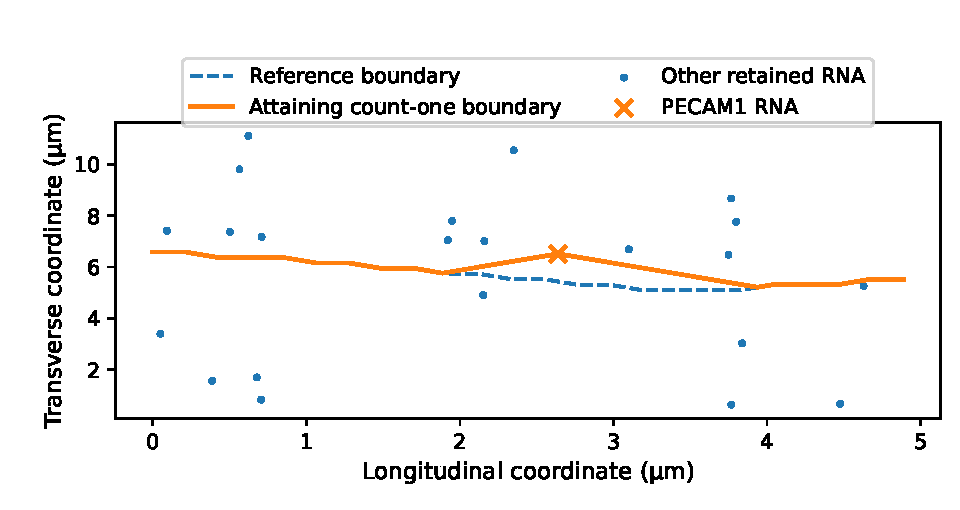
\includegraphics[width=\textwidth]{figures/native_count_witness.pdf}
\caption{Native-derived two-cell example. The solid curve attains a PECAM1 count of one in the lower-side cell; the dashed curve is the reference. Other transcripts remain in the shared model. This is a fitted local corridor, not a whole-cell reconstruction.}\label{fig:suppnative}
\end{figure}
\section{Overlap audit and union-of-one-corridor semantics}
The original 14,384 interval rows yield 11,392 distinct region/setting/cell/gene/budget keys after dropping the corridor field. Exactly 178 keys have unequal intervals across their constituent corridors: 74 baseline and 104 enlarged. Nineteen of 51 cells occur in multiple corridors, up to seven per cell. For cell 153131 and CD8A at area $1\,\mu$m$^2$, corridor 02d9a53ef82968 gives $[2,2]$, while 4c4f466415dd22 gives $[2,3]$, in both settings. These are quantified statements about different feasible sets.

For a fixed region, setting, cell and gene, define a union family that permits any one of the declared corridors to vary and otherwise retains the source. The exact outer endpoints for this family are the minimum of the constituent lower endpoints and maximum of the upper endpoints, with source-only counts for corridors leaving this entry unchanged. This follows directly by optimizing over a union. An endpoint witness identifies which constituent family attains it. The construction resolves the indexing ambiguity for a choice of one local intervention; it supplies no simultaneous-edit, entire-cell or whole-tissue guarantee. Geometric overlaps and repeated transcript IDs are rejected by the independent-patch composition interface.

\section{Executed Proseg development-crop comparison}
Proseg 3.2.0 \cite{proseg} was executed on both supplied development crops. The initial default-factorization run on the first crop failed with an empty-input error during feature selection, reproduced from Parquet and equivalent CSV inputs. We disabled factorization for both crops after this failure, before comparing their assignments. Remaining model and sampler settings used upstream defaults: 200 burn-in iterations, 200 sampling iterations and 50 hill-climb steps, with two requested CPU threads. Diffusion and source reassignment remained enabled. One stochastic run was retained per crop; this version exposes no random-seed argument.

\begin{center}
\begin{tabular}{lrr}\toprule
Quantity & Crop 1 & Crop 2\\\midrule
Supplied transcripts &5,847&1,523\\
Proseg-retained transcripts &5,774&1,482\\
Excluded transcripts &73&41\\
Proseg output cells &93&72\\
Different owner from source &3,242&765\\
Proseg unassigned/background &2,484&1,335\\
Changed active cell/gene counts &2,794&590\\\bottomrule
\end{tabular}
\end{center}

Comparison joins exact transcript IDs and maps output cell IDs through the original-cell mapping. Gene and XY consistency are checked; excluded IDs are retained explicitly. The source masks are a comparison reference rather than molecular truth. Crops truncate cells and omit surrounding tissue; cells without retained nuclear transcripts may be absent at initialization. The large background assignment fraction especially in crop 2 makes these inputs inadequate for a strong field benchmark. These adapted executions demonstrate a functioning external-method adapter and recorded assignment differences, without estimating accuracy, uncertainty coverage or biological improvement. The artifact retains commands, binary and data hashes, complete outputs and the failed default-run log. This experiment adds neither a donor nor external validation of the corridor family.

\section{Evidence boundary}
The native analysis contains one biological specimen. Generated calibration units are independent draws from the programmed piecewise-linear family and therefore test software behavior under that model. They cannot validate its anatomical adequacy. A separate external raster audit exists in the continuation materials, but concerns a different family and RNA-informed reference masks; its count coverage is not validation of this continuum theorem. An external test of the exact family would require fixed extraction rules, independently measured boundary references, training/calibration units separate from evaluation units, and reporting geometric containment alongside count coverage and useful interval widths.

\begin{thebibliography}{99}
\bibitem{baysor} V. Petukhov et al. Cell segmentation in imaging-based spatial transcriptomics. \emph{Nature Biotechnology} 40, 345--354 (2022). doi:10.1038/s41587-021-01044-w.
\bibitem{proseg} D. C. Jones et al. Cell simulation as cell segmentation. \emph{Nature Methods} 22, 1331--1342 (2025). doi:10.1038/s41592-025-02697-0.
\bibitem{resolvi} C. Ergen and N. Yosef. ResolVI: addressing noise and bias in spatial transcriptomics. \emph{Nature Methods} 23, 2003--2014 (2026). doi:10.1038/s41592-026-03212-9.
\bibitem{tissue} E. D. Sun, R. Ma, P. Navarro Negredo, A. Brunet and J. Zou. TISSUE: uncertainty-calibrated prediction of single-cell spatial transcriptomics improves downstream analyses. \emph{Nature Methods} 21, 444--454 (2024). doi:10.1038/s41592-024-02184-y.
\bibitem{li} K. Li, X. Wu, D. Z. Chen and M. Sonka. Optimal surface segmentation in volumetric images---a graph-theoretic approach. \emph{IEEE TPAMI} 28, 119--134 (2006). doi:10.1109/TPAMI.2006.19.
\bibitem{shah} A. Shah, M. D. Abramoff and X. Wu. Optimal surface segmentation with convex priors in irregularly sampled space. \emph{Medical Image Analysis} 54, 63--75 (2019). doi:10.1016/j.media.2019.02.004.
\bibitem{kolmogorov} V. Kolmogorov and R. Zabih. What energy functions can be minimized via graph cuts? \emph{IEEE TPAMI} 26, 147--159 (2004). doi:10.1109/TPAMI.2004.1262177.
\bibitem{conformal} A. N. Angelopoulos and S. Bates. A gentle introduction to conformal prediction and distribution-free uncertainty quantification. arXiv:2107.07511.
\bibitem{picard} J. C. Picard and M. Queyranne. On the structure of all minimum cuts in a network and applications. \emph{Mathematical Programming Study} 13, 8--16 (1980).
\bibitem{gallo} G. Gallo, M. D. Grigoriadis and R. E. Tarjan. A fast parametric maximum flow algorithm and applications. \emph{SIAM Journal on Computing} 18, 30--55 (1989). doi:10.1137/0218003.
\bibitem{papandreou} G. Papandreou and A. L. Yuille. Perturb-and-MAP random fields: using discrete optimization to learn and sample from energy models. \emph{ICCV} (2011). Author material: \url{https://home.ttic.edu/~gpapan/research/perturb_and_map/}.
\bibitem{dataset} 10x Genomics. Preview data: FFPE human lung cancer with Xenium multimodal cell segmentation (2024). One-donor public dataset, CC BY 4.0. \url{https://www.10xgenomics.com/datasets/preview-data-ffpe-human-lung-cancer-with-xenium-multimodal-cell-segmentation-1-standard}.
\bibitem{ishikawa} H. Ishikawa. Exact optimization for Markov random fields with convex priors. \emph{IEEE TPAMI} 25(10):1333--1336, 2003. doi:10.1109/TPAMI.2003.1233908.
\bibitem{hochbaum} D. S. Hochbaum. An efficient algorithm for image segmentation, Markov random fields and related problems. \emph{Journal of the ACM} 48(4):686--701, 2001.
\bibitem{kohli} P. Kohli, L. Ladick\'{y} and P. H. S. Torr. Robust higher order potentials for enforcing label consistency. \emph{International Journal of Computer Vision} 82:302--324, 2009. doi:10.1007/s11263-008-0202-0.
\end{thebibliography}
\end{document}
